% This file is based on the "sig-alternate.tex" V1.9 April 2009
% This file should be compiled with V2.4 of "sig-alternate.cls" April 2009

\documentclass{sig-alternate}

\usepackage{graphicx}
\usepackage{url}
\usepackage{color}
\usepackage{enumerate}
\usepackage{balance}
\permission{}
\CopyrightYear{2013}

\usepackage[english]{babel}
\usepackage{blindtext}

\usepackage{etoolbox}
\makeatletter
\patchcmd{\maketitle}{\@copyrightspace}{}{}{}
\makeatother

%\crdata{0-00000-00-0/00/00}
\begin{document}

%%% Maketitle metadata
\newcommand{\horrule}[1]{\rule{\linewidth}{#1}} 	% Horizontal rule

\title{
		%\vspace{-1in} 	
		\usefont{OT1}{bch}{b}{n}
		\normalfont \normalsize \textsc{Rochester Institute of Technology} \\ [25pt]
		\horrule{0.5pt} \\[0.4cm]
		\huge What Should I Wear \\
		\horrule{2pt} \\[0.5cm]
		\vspace{-10mm}
}

\author{
		\normalfont 								\normalsize 
        Piter Garcia and Anthony Castiglia\\[-3pt]		\normalsize
        \today
}
\date{}
\maketitle
\begin{abstract}

The aim of this project is to learn and implement the techniques of Data Cleaning and Preparation for data mining. In this project, we would be using weather data sets from various locations of the United States to show the weather trends in a particular area and use them for prediction. In particular, Data Mining techniques will be used to analyse past weather patterns for different locations and predict, for example, whether or not a person should wear a coat or shorts depending on the weather trends. We are going to design an interface for people who need help in deciding what to wear when planning a trip. The input of this would be taken from users, such as the approximate dates they would be going on a trip and the city as well.

\end{abstract}
\vspace{5 mm}

\section{Overview}
\label{overview}

The dataset consists of temperature and precipitation of multiple cities from different areas of the United States. The website that we are obtaining these datasets from has been
collecting weather data from these areas for the past 54 years. The large collection of data will definitely help us in finding the weather trends of a city and making our results more reliable. The aim of this project is to obtain the cleanest data possible to make querying for weather information and suggestions easy and reliable.
\newline

Our main goal is to make querying for the weather information easy and reliable. This can be accomplished through our software application by taking the input of users and providing them with a graphical output that can be easily interpreted.



\section{Design Considerations}
\label{design considerations}

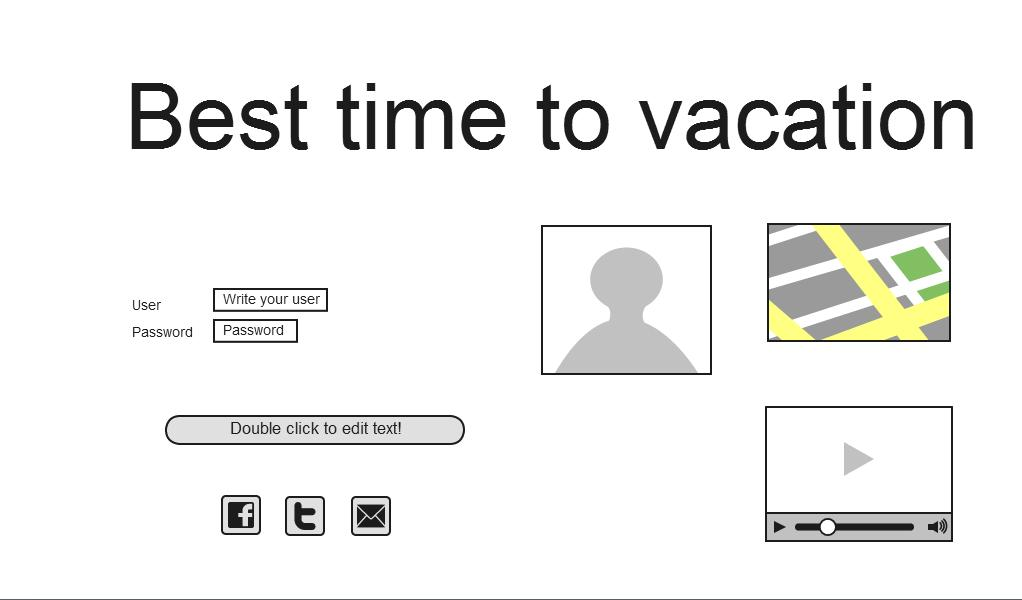
\includegraphics[scale=0.2]{design.eps} 

We have designed a website design of what we would like to be the platform to shape and implement our project according to our expectations. In order to fulfill the design and
project patterns we are going to break down our approach in two sections. This will give the reader a better insight about our approach to build our system. The section 3 and session 4 better explain the structure of our project design. The section 3 explains how our database was obtained and how it is being used for our objective of the project. The section 4 explains how this database is implemented and developed towards the objective of our project. Finally, section 5 gives an update and better understanding of how close we are from reaching the goal of our project.


\subsection{Database Design}
\includegraphics[scale=0.2]{design2.eps} 
\newline The image above is an example of how we would like the interface to interact with our database. This design is subjected to changes as we are still in the cleaning and preparation process of our database. This design is subjected to changes as we are still in the cleaning and preparation process of our database.\newline


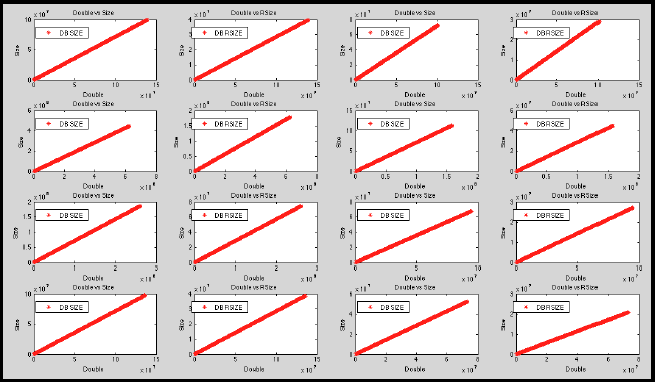
\includegraphics[scale=0.17]{fir.eps} 
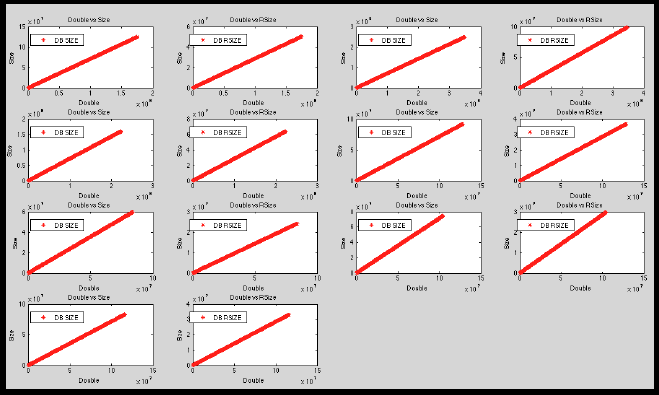
\includegraphics[scale=0.165]{sec.eps} 
\newline Currently, we have reduced the amount of data we have, obtained from the online source cited below, due to our current design.  The reasons to this are the followings: First, we do not believe that more than 20 years of data is necessary to achieve the goal of this project. Second, the cleaning and preparation process of the data is taking too
long because the data sets are too big for our computer processors to handle. Finally, the two images above is a comparison between our database before and after shrinking the data
sets to 20 years of data. In order to do this, we used a Java program that we coded specifically for our database, which has been attached to the report.
\newline

We have also coded a Java program to modify the datasets according to our design. For our design it was necessary for us to have the average temperature as well as a class that specifies a level of approximation as to how cold or hot the place is. This would make it easier for us when applying normalization techniques to make datasets comparison much easier. Furthermore, we used R to test one of our dataset to observe its behavior when being normalized by an artificial neural network transfer function simulation. This is what we are originally using to create our overall database model and has precluded us from gathering weather datasets from 2000 until 2012. On the other hand, we will proceed to collect the necessary weather information from the time period mentioned above to obtain the dataset and include it in our database once our prototype is working as desired.
\newline

Dataset Model\newline
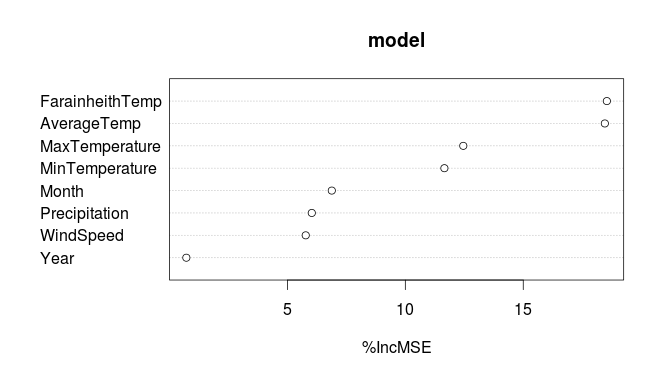
\includegraphics[scale=0.3]{phase1-Model.eps} 
\section{Architecture}
\label{architecture}

The structure of the interface implementation has not been utterly decided yet because our main focus, as right now, is the cleaning and preparation of the data for mining purpose. Nevertheless, we are considering to make use of PHP, HTML and MySQL programming tools to handle the data. Other programming tools such as Java and C++ to decode and reduce our data set as part of the preparation process before applying the techniques to learn for the data cleaning process. This is the process that will remove unwanted information such as noisy, repeated and not useful values to make the data useful for data mining. Moreover, we are planning to develop our own interface to allow users to interact with our underlying engine . In order to achieve this, cleaning techniques must be applied to convert all datasets into an usable and more meaningful database, and to remove all unwanted information to make the data more practical for the application while avoiding delays.



\section{Implementation}
\label{implementation}

The implementation of our project takes place once the weather and precipitation from most cities of the United States is cleaned and prepared for data mining. This data is used for analysis purpose to give the user an advice on what should be wearing based on the weather trends that have previously happened in a place of the user choice. We would like to take the datasets of the cities along with the user dataset to create another dataset that only contains cities that users in a cluster may like based on their behavior.

\section{Current Status}
\label{current status}

We have gathered weather information of multiple locations of the United States for our database. This weather has been collected from 1980 till 2000, we most emphasize that collecting these datasets has been time consuming and has precluded us from gathering weather datasets from 2000 until 2012. However, we will proceed to collect the necessary weather information from the time period mentioned above to obtain the dataset and include it in our database once our prototype is working as desired.
\newline\newline
Classification of the Dataset\newline
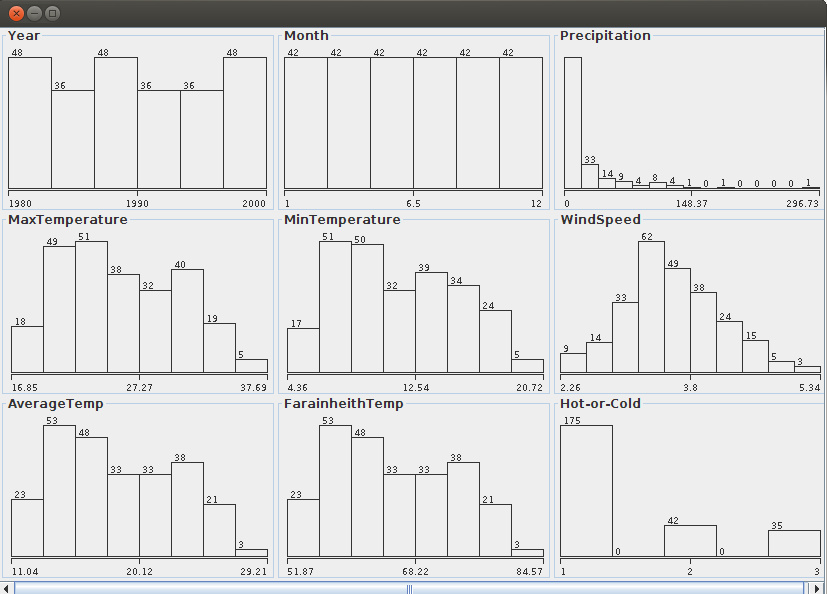
\includegraphics[scale=0.2]{phase1.eps} 
\newline\newline
Cluster Analysis of the Dataset\newline
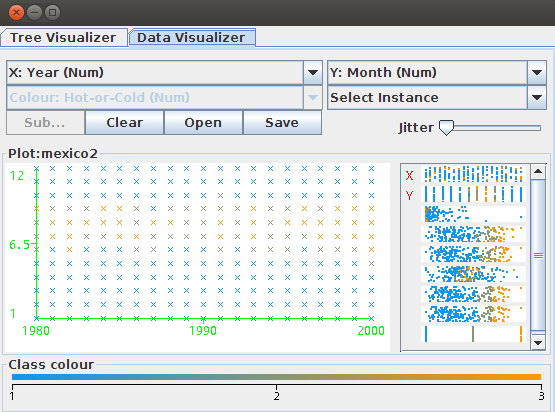
\includegraphics[scale=0.3]{phase1-2.eps} 
\newline

Besides the database model work explained in the "Data Design" section, we have done some analysis of one of the datasets in WEKA to give a visual representation of data. This visual representation, shown above, is the visual representation of what was ex- plained in the tables response obtained from the work done in the "Data Design" section.
\newline 

We have actually developed an interface design for the platform where all this data manipulation and managing is to take place. All datasets that have been downloaded and are currently on a cleaning process to prepare them and make them usable for our SQL database.
\newline 

\section{Future Status}
\label{Future status}
The future work required can be categorized in the following three sections:

\begin{itemize}

	\item Big Data:\newline
	We need to design a system that asks users to designate a time range and a city. This 		way we can systematically can advice users on a wearing a coat or not,for example, by 		obtaining the weather approximation based on the past temperature, precipitation other
 	weather information.
 \newline
	
	\begin{itemize}
		\item 
		More research is needed to improve the ability to blend different datasets into an 		integrated system.
		
		\item 
		Data could be assimilated into different models.
	\end{itemize}
	
	\item Data Mining:\newline
	We are planning to develop an extra feature for our application. This feature will be 		based on users previous selected locations to prioritize the list of suggested places 		that users may like based on our system users overall behavior.

	\begin{itemize}
		\item 
		Develop an interface to allow users to easily input the dates or their trip and 	  		city to determine whether they should wear a coat, and or shorts, or not.
		
		\item 
		Apply data mining techniques to develop a list of suggested cities based on the 				users search behaviour and profile information.
		
		\item 
		Create systems for control and feedback, proper data archival and access, and 				sustained data management systems.
	\end{itemize}
	
\end{itemize}

\section{Table}
\label{Table}
The tables attached to this phase report contain only weather information of one of the file from one of the areas in our data set. These images are only to show the response obtained from R when processing our datasets through a transfer function that simulates a an artificial neural network, as well as understanding the data with WEKA analysis techniques. More testing is required to make sure that our data is indeed reasonable and useful. It is important to highlight that each one of the area station contains huge datasets. Therefore, it would be impossible for us to attach their respective files because of the large size of their data that includes the respected area cities weather information. Therefore, I have attached a link to access all datasets and zip file that contains the information of our datasets, in a file named "Reed Me - Dataset Description", including this report.
\newline

Table 1: R Analysis
\newline
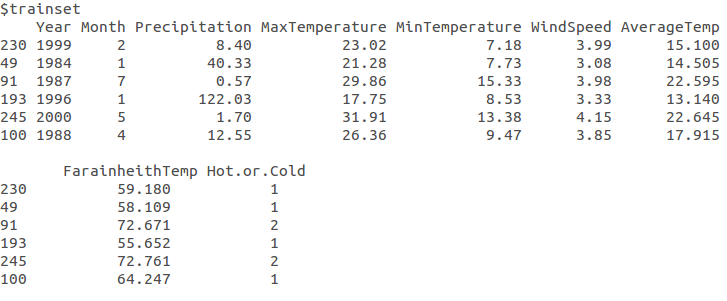
\includegraphics[scale=0.3]{tr1.eps}
\newline\newline\newline\newline\newline 

Table 2: R Analysis
\newline
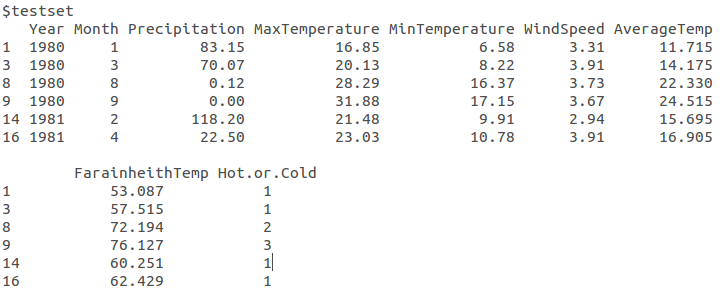
\includegraphics[scale=0.3]{tr2.eps}
\newline
\section{References}

[1] NCDC. Babel, Whether Datasets. cdo-web,
	12(2):291–301, June 1991.
	http://www.ncdc.noaa.gov/cdo-web/
\newline

[2] M. Clark. Post congress tristesse. In TeX90 Conference
	Proceedings, pages 84–89. TeX Users Group, March1991.
\newline

[3] M. Herlihy. A methodology for implementing highly
	concurrent data objects. ACM Trans. Program. Lang.
	Syst., 15(5):745–770, November 1993.
\newline

\end{document}








